\documentclass[10pt,a4paper]{article}
\usepackage[margin=0.6in]{geometry}
\usepackage{amsmath,amssymb,amsthm}
\usepackage{booktabs}
\usepackage{multirow}
\usepackage{xcolor}
\usepackage{tcolorbox}
\tcbuselibrary{breakable}
\usepackage[colorlinks=true,linkcolor=blue]{hyperref}
\usepackage{titlesec}
\usepackage{enumitem}
\usepackage{tikz}
\usepackage{circuitikz}
\usetikzlibrary{shapes,arrows,positioning,calc,decorations.pathmorphing}

% Color scheme
\definecolor{headcolor}{RGB}{0,102,204}
\definecolor{keycolor}{RGB}{220,20,60}
\definecolor{solutioncolor}{RGB}{34,139,34}
\definecolor{mnemoniccolor}{RGB}{148,0,211}

% Custom environments
\newtcolorbox{solutionbox}{
 breakable,
 colback=solutioncolor!5!white,
 colframe=solutioncolor!75!black,
 fonttitle=\bfseries,
 title=Answer
}

\newtcolorbox{keyformula}{
 colback=keycolor!5!white,
 colframe=keycolor!75!black,
 fonttitle=\bfseries,
 title=Key Formula
}

\newtcolorbox{mnemonicbox}{
 colback=mnemoniccolor!5!white,
 colframe=mnemoniccolor!75!black,
 fonttitle=\bfseries,
 title=Mnemonic
}

% Spacing
\setlength{\parskip}{3pt}
\setlist[itemize]{nosep}
\setlist[enumerate]{nosep}

% Title formatting
\titleformat{\section}{\Large\bfseries\color{headcolor}}{\thesection}{1em}{}
\titleformat{\subsection}{\large\bfseries\color{headcolor}}{\thesubsection}{1em}{}

\begin{document}

\begin{center}
{\Huge\bfseries\color{headcolor} Fundamentals of Electrical Engineering}\\[5pt]
{\LARGE DI01000101 -- Winter 2024}\\[3pt]
{\large Semester 1 Study Material}\\[3pt]
{\normalsize\textit{Detailed Solutions and Explanations}}
\end{center}

\vspace{10pt}

%----------------------------------------
\section*{Question 1(a) [3 marks]}
\textbf{Explain Ohm's law with its limitation and application.}

\begin{solutionbox}
\textbf{Ohm's Law Summary:}

\begin{center}
\begin{tabular}{|l|p{8cm}|}
\hline
\textbf{Aspect} & \textbf{Description} \\
\hline
Statement & Current through a conductor is directly proportional to voltage across it, provided physical conditions remain constant. \\
\hline
Formula & $V = I \times R$ \\
\hline
Units & $V$ (Volts), $I$ (Amperes), $R$ (Ohms) \\
\hline
\end{tabular}
\end{center}

\textbf{Limitations:}
\begin{itemize}
\item \textbf{Temperature dependency}: Resistance changes with temperature.
\item \textbf{Non-linear materials}: Does not apply to semiconductors, diodes, etc.
\item \textbf{AC circuits}: Modified form needed for reactive components (Impedance $Z$).
\end{itemize}

\textbf{Applications:}
\begin{itemize}
\item \textbf{Circuit analysis}: Calculate unknown voltage, current, or resistance.
\item \textbf{Power calculations}: $P = V^2/R$ or $P = I^2R$.
\end{itemize}
\end{solutionbox}

\begin{mnemonicbox}
``Voltage Is Really Important'' ($V = I \times R$)
\end{mnemonicbox}

%----------------------------------------
\section*{Question 1(b) [4 marks]}
\textbf{Explain Faraday's law of electromagnetic induction with necessary figure.}

\begin{solutionbox}
\textbf{Faraday's Laws:}
\begin{itemize}
\item \textbf{First Law}: An EMF is induced in a conductor whenever the magnetic flux linking with it changes.
\item \textbf{Second Law}: The magnitude of the induced EMF is equal to the rate of change of flux linkages.
\end{itemize}

\begin{keyformula}
\[e = -N \frac{d\Phi}{dt}\]
\end{keyformula}

\textbf{Diagram:}
\begin{center}
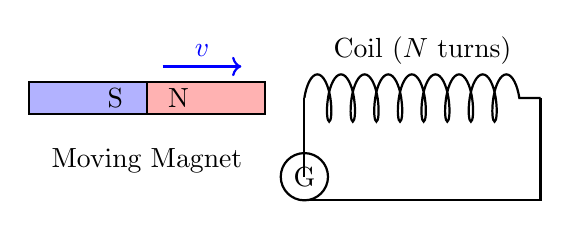
\begin{tikzpicture}[scale=1.0]
% Coil
\draw[thick, decoration={aspect=0.3, segment length=3mm, amplitude=3mm,coil},decorate] (0,0) -- (3,0); 
\draw[thick] (0,0) -- (0,-1);
\draw[thick] (3,0) -- (3,-1);
\node at (1.5,0.6) {Coil ($N$ turns)};
% Galvanometer
\draw[thick] (0,-1) circle (0.3);
\node at (0,-1) {G};
\draw[thick] (0,-1.3) -- (3,-1.3) -- (3,-1);

% Magnet
\draw[thick, fill=red!30] (-2, -0.2) rectangle (-0.5, 0.2);
\node at (-1.6, 0) {N};
\draw[thick, fill=blue!30] (-3.5, -0.2) rectangle (-2, 0.2);
\node at (-2.4, 0) {S};
\draw[->, thick, blue] (-1.8, 0.4) -- (-0.8, 0.4) node[midway, above] {$v$};

\node at (-2, -0.8) {Moving Magnet};
\end{tikzpicture}
\end{center}

\textbf{Applications:}
\begin{itemize}
\item \textbf{Transformers}: Mutual induction principle.
\item \textbf{Generators}: Mechanical to electrical energy conversion.
\end{itemize}
\end{solutionbox}

\begin{mnemonicbox}
``Flux Change Generates EMF'' ($d\Phi/dt = \text{EMF}$)
\end{mnemonicbox}

%----------------------------------------
\section*{Question 1(c) [7 marks]}
\textbf{Explain Kirchhoff's Voltage Law (KVL) and Kirchhoff's Current Law (KCL) with necessary diagram.}

\begin{solutionbox}
\textbf{Comparison:}
\begin{center}
\begin{tabular}{|l|p{4cm}|c|l|}
\hline
\textbf{Law} & \textbf{Statement} & \textbf{Formula} & \textbf{Application} \\
\hline
KVL & Sum of voltages in closed loop is zero & $\sum V = 0$ & Series circuits \\
\hline
KCL & Sum of currents at a node is zero & $\sum I = 0$ & Parallel circuits \\
\hline
\end{tabular}
\end{center}

\textbf{KVL Diagram:}
\begin{center}
\begin{circuitikz}[scale=0.8]
\draw (0,0) to[battery1, l=$V_1$] (0,3)
      to[R, l=$R_1$] (3,3)
      to[battery1, l=$V_2$] (3,0)
      to[R, l=$R_2$] (0,0);
\draw[->] (1,1.5) arc (-60:240:0.5) node[midway, below] {$Loop$};
\end{circuitikz}
\end{center}

\textbf{KCL Diagram:}
\begin{center}
\begin{circuitikz}[scale=0.8]
\draw (0,0) node[circ, label={Node $N$}] (N) {};
\draw[<-] (N) -- ++(-1.5,1) node[left] {$I_1$};
\draw[<-] (N) -- ++(0,1.5) node[above] {$I_2$};
\draw[->] (N) -- ++(1.5,1) node[right] {$I_3$};
\draw[->] (N) -- ++(0,-1.5) node[below] {$I_4$};
\end{circuitikz}
\end{center}

\textbf{Key Points:}
\begin{itemize}
\item \textbf{KVL}: Algebraic sum considers voltage polarities.
\item \textbf{KCL}: Considers current directions (incoming = positive, outgoing = negative).
\end{itemize}
\end{solutionbox}

\begin{mnemonicbox}
``Voltage Loops, Current Nodes''
\end{mnemonicbox}

%----------------------------------------
\section*{Question 1(c OR) [7 marks]}
\textbf{Differentiate statically induced EMF and dynamically induced EMF.}

\begin{solutionbox}
\begin{center}
\begin{tabular}{|l|p{5cm}|p{5cm}|}
\hline
\textbf{Parameter} & \textbf{Statically Induced EMF} & \textbf{Dynamically Induced EMF} \\
\hline
Cause & Changing magnetic field & Relative motion between conductor and field \\
\hline
Field & Time-varying, conductor stationary & Steady field, conductor moving \\
\hline
Examples & Transformer, Inductor & Generator, Motor \\
\hline
Formula & $e = -N \frac{d\Phi}{dt}$ & $e = B l v \sin\theta$ \\
\hline
Applications & AC circuits, power supplies & Power generation, motors \\
\hline
\end{tabular}
\end{center}

\textbf{Static EMF Types:}
\begin{itemize}
\item \textbf{Self-induced}: EMF in the same coil due to its own flux change.
\item \textbf{Mutually induced}: EMF in a coil due to flux change in a neighboring coil.
\end{itemize}
\end{solutionbox}

\begin{mnemonicbox}
``Static Stays, Dynamic Dances''
\end{mnemonicbox}

%----------------------------------------
\section*{Question 2(a) [3 marks]}
\textbf{Explain various types of losses in transformer.}

\begin{solutionbox}
\begin{center}
\begin{tabular}{|l|l|p{3cm}|p{4cm}|}
\hline
\textbf{Loss Type} & \textbf{Cause} & \textbf{Location} & \textbf{Characteristics} \\
\hline
\textbf{Iron Loss} & Hysteresis + Eddy currents & Core & Constant, frequency dependent \\
\hline
\textbf{Copper Loss} & $I^2R$ heating & Windings & Variable with load ($I^2$) \\
\hline
\textbf{Stray Loss} & Leakage flux & Overall & Minimal \\
\hline
\end{tabular}
\end{center}

\textbf{Details:}
\begin{itemize}
\item \textbf{Hysteresis loss}: Due to magnetic domain reversal energy.
\item \textbf{Eddy current loss}: Due to circulating currents in the core (reduced by lamination).
\item \textbf{Copper loss}: Depends on current, proportional to square of load current.
\end{itemize}
\end{solutionbox}

\begin{mnemonicbox}
``Iron Core, Copper Coil''
\end{mnemonicbox}

%----------------------------------------
\section*{Question 2(b) [4 marks]}
\textbf{Explain working principle of transformer.}

\begin{solutionbox}
\textbf{Working Principle:} Mutual electromagnetic induction between primary and secondary windings linked by a common magnetic core.

\textbf{Diagram:}
\begin{center}
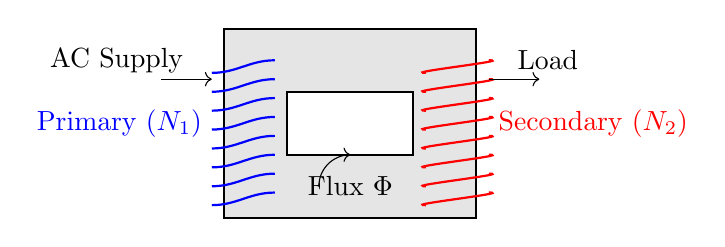
\begin{tikzpicture}[scale=0.8]
% Core
\draw[thick, fill=gray!20] (0,0) rectangle (4,3);
\draw[thick, fill=white] (1,1) rectangle (3,2);

% Primary
\foreach \y in {0.2,0.5,0.8,1.1,1.4,1.7,2.0,2.3}
    \draw[thick, blue] (-0.2,\y) to[out=0,in=180] (0.8,\y+0.2);
\node[left, blue] at (-0.2, 1.5) {Primary ($N_1$)};
\node[left] at (-0.5, 2.5) {AC Supply};
\draw[->] (-1, 2.2) -- (-0.2, 2.2);

% Secondary
\foreach \y in {0.2,0.5,0.8,1.1,1.4,1.7,2.0,2.3}
    \draw[thick, red] (3.2,\y) to[out=180,in=0] (4.2,\y+0.2);
\node[right, red] at (4.2, 1.5) {Secondary ($N_2$)};
\node[right] at (4.5, 2.5) {Load};
\draw[->] (4.2, 2.2) -- (5, 2.2);

\node at (2, 0.5) {Flux $\Phi$};
\draw[->] (1.5, 0.5) arc (180:90:0.5);
\end{tikzpicture}
\end{center}

\textbf{Operation Steps:}
\begin{enumerate}
\item AC current in primary creates alternating flux.
\item Flux circulates through the magnetic core.
\item Flux links with secondary winding.
\item Changing flux induces EMF in secondary (Faraday's Law).
\end{enumerate}

\begin{keyformula}
\[\frac{V_2}{V_1} = \frac{N_2}{N_1} = \frac{I_1}{I_2} = K\]
\end{keyformula}
\end{solutionbox}

\begin{mnemonicbox}
``Primary Produces, Secondary Supplies''
\end{mnemonicbox}

%----------------------------------------
\section*{Question 2(c) [7 marks]}
\textbf{Derive EMF equation of transformer.}

\begin{solutionbox}
\textbf{Given:}
\begin{itemize}
\item $N_1, N_2$: Number of turns
\item $\Phi_m$: Maximum flux in core
\item $f$: Frequency of supply
\end{itemize}

\textbf{Derivation:}
\begin{enumerate}
\item \textbf{Flux Equation}: $\Phi = \Phi_m \sin(2\pi f t)$
\item \textbf{Induced EMF}: $e = -N \frac{d\Phi}{dt}$
\item \textbf{Differentiation}:
\[e = -N \frac{d}{dt}(\Phi_m \sin(2\pi f t)) = -N \Phi_m (2\pi f) \cos(2\pi f t)\]
\[e = 2\pi f N \Phi_m \sin(2\pi f t - 90^\circ)\]
\item \textbf{Maximum EMF}: $E_m = 2\pi f N \Phi_m$
\item \textbf{RMS EMF}: $E_{rms} = \frac{E_m}{\sqrt{2}} = \frac{2\pi f N \Phi_m}{\sqrt{2}} = 4.44 f N \Phi_m$
\end{enumerate}

\begin{keyformula}
\[E_1 = 4.44 f N_1 \Phi_m \quad \text{and} \quad E_2 = 4.44 f N_2 \Phi_m\]
\end{keyformula}

\textbf{Transformation Ratio:} $K = \frac{E_2}{E_1} = \frac{N_2}{N_1}$
\end{solutionbox}

\begin{mnemonicbox}
``4.44 Flux Formula''
\end{mnemonicbox}

%----------------------------------------
\section*{Question 2(a OR) [3 marks]}
\textbf{Write application of transformer.}

\begin{solutionbox}
\begin{center}
\begin{tabular}{|l|p{4cm}|l|}
\hline
\textbf{Application} & \textbf{Purpose} & \textbf{Voltage Level} \\
\hline
Power Transmission & Reduce transmission losses ($I^2R$) & Step-up (e.g., 400 kV) \\
\hline
Distribution & Safe voltage for consumers & Step-down (e.g., 230 V) \\
\hline
Isolation & Electrical safety/isolation & 1:1 Ratio \\
\hline
Electronics & DC power supplies & Step-down \\
\hline
\end{tabular}
\end{center}

\textbf{Industrial Uses:} Welding transformers (High Current), Instrument transformers (CT/PT).
\end{solutionbox}

\begin{mnemonicbox}
``Power Distribution Isolation Electronics''
\end{mnemonicbox}

%----------------------------------------
\section*{Question 2(b OR) [4 marks]}
\textbf{Write equation for back EMF and torque of D.C motor.}

\begin{solutionbox}
\textbf{1. Back EMF Equation:}
\[E_b = \frac{\phi Z N P}{60 A}\]
Simplified: $E_b = K \phi N$

\textbf{2. Torque Equation:}
\[T = \frac{\phi Z I_a P}{2\pi A}\]
Simplified: $T = K \phi I_a$

\textbf{Where:}
\begin{itemize}
\item $\phi$: Flux per pole (Weber)
\item $Z$: Total armature conductors
\item $N$: Speed (RPM)
\item $P$: Number of poles
\item $A$: Parallel paths
\item $I_a$: Armature current
\end{itemize}
\end{solutionbox}

\begin{mnemonicbox}
``Back EMF opposes, Torque proposes''
\end{mnemonicbox}

%----------------------------------------
\section*{Question 2(c OR) [7 marks]}
\textbf{Explain construction and working of D.C. motor with necessary figure.}

\begin{solutionbox}
\textbf{Construction:}
\begin{itemize}
\item \textbf{Stator}: Yoke, Poles, Field windings (Produces magnetic field).
\item \textbf{Rotor (Armature)}: Stacked laminations with slots for conductors.
\item \textbf{Commutator}: Split rings to reverse current direction.
\item \textbf{Brushes}: Carbon brushes to collect/supply current.
\end{itemize}

\textbf{Diagram:}
\begin{center}
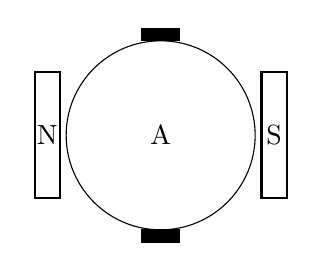
\begin{tikzpicture}[scale=0.8]
\draw (0,0) circle (1.5); % Armature
\node at (0,0) {A};
\draw[thick] (-2, -1) rectangle (-1.6, 1); % Pole N
\node at (-1.8, 0) {N};
\draw[thick] (1.6, -1) rectangle (2, 1); % Pole S
\node at (1.8, 0) {S};
% Brushes
\draw[fill=black] (-0.3, 1.5) rectangle (0.3, 1.7);
\draw[fill=black] (-0.3, -1.7) rectangle (0.3, -1.5);
\end{tikzpicture}
\end{center}

\textbf{Working Principle:}
\begin{enumerate}
\item Current flows through armature conductors placed in a magnetic field.
\item A mechanical force is experienced (Lorentz Force $F = BIl$).
\item Forces on opposite sides produce a torque.
\item Commutator reverses current direction every half rotation to maintain unidirectional torque.
\end{enumerate}
\end{solutionbox}

\begin{mnemonicbox}
``Current Creates Circular Motion''
\end{mnemonicbox}

%----------------------------------------
\section*{Question 3(a) [3 marks]}
\textbf{Explain construction of transformer.}

\begin{solutionbox}
\textbf{Core Components:}
\begin{center}
\begin{tabular}{|l|l|p{5cm}|}
\hline
\textbf{Component} & \textbf{Material} & \textbf{Function} \\
\hline
Core & Silicon Steel & Provides low reluctance magnetic path. Laminated to reduce eddy currents. \\
\hline
Windings & Copper/Aluminium & Primary carries input, Secondary carries output current. \\
\hline
Insulation & Paper/Varnish & Prevents short circuits. \\
\hline
Tank & Steel & Protection and cooling (oil filled). \\
\hline
\end{tabular}
\end{center}

\textbf{Types:} Core Type (Windings surround core), Shell Type (Core surrounds windings).
\end{solutionbox}

\begin{mnemonicbox}
``Core Carries Current Carefully''
\end{mnemonicbox}

%----------------------------------------
\section*{Question 3(b) [4 marks]}
\textbf{Explain application of DC motor.}

\begin{solutionbox}
\begin{center}
\begin{tabular}{|l|p{3cm}|p{5cm}|}
\hline
\textbf{Motor Type} & \textbf{Characteristics} & \textbf{Applications} \\
\hline
Shunt Motor & Constant Speed & Lathes, Fans, Centrifugal Pumps, Machine Tools \\
\hline
Series Motor & High Starting Torque & Traction (Trains), Cranes, Hoists \\
\hline
Compound Motor & Stable Speed \& Torque & Elevators, Compressors, Rolling Mills \\
\hline
\end{tabular}
\end{center}
\end{solutionbox}

\begin{mnemonicbox}
``Shunt Stays, Series Speeds''
\end{mnemonicbox}

%----------------------------------------
\section*{Question 3(c) [7 marks]}
\textbf{Explain different types of DC motor.}

\begin{solutionbox}
\textbf{Classification based on Field Connection:}

\begin{enumerate}
\item \textbf{DC Shunt Motor}:
\begin{itemize}
\item Field winding connected in parallel with armature.
\item Constant speed motor.
\end{itemize}
\begin{center}
\begin{circuitikz}[scale=0.7]
\draw (0,0) to[short] (2,0) to[short] (2,1) to[R, l=$R_{sh}$] (2,3) to[short] (2,4) to[short] (0,4);
\draw (2,0) to[short] (4,0) to[short] (4,1) to[rmeter, t=M, l=$R_a$] (4,3) to[short] (4,4) to[short] (2,4);
\draw (0,0) to[short] (-1,0) node[below] {$-$};
\draw (0,4) to[short] (-1,4) node[above] {$+$};
\node at (-1, 2) {$V_{dc}$};
\end{circuitikz}
\end{center}

\item \textbf{DC Series Motor}:
\begin{itemize}
\item Field winding connected in series with armature.
\item Application: High starting torque loads.
\end{itemize}

\item \textbf{DC Compound Motor}:
\begin{itemize}
\item Contains both series and shunt field windings.
\end{itemize}
\end{enumerate}

\begin{keyformula}
Shunt: $N \propto \frac{V - I_a R_a}{\phi}$ \quad Series: $N \propto \frac{V}{\sqrt{T}}$
\end{keyformula}
\end{solutionbox}

\begin{mnemonicbox}
``Shunt Steady, Series Strong, Compound Combined''
\end{mnemonicbox}

%----------------------------------------
\section*{Question 3(a OR) [3 marks]}
\textbf{Explain transformation ratio of transformer.}

\begin{solutionbox}
\textbf{Definition}: The ratio of secondary voltage (or turns) to primary voltage (or turns).

\begin{keyformula}
\[K = \frac{N_2}{N_1} = \frac{E_2}{E_1} = \frac{V_2}{V_1} = \frac{I_1}{I_2}\]
\end{keyformula}

\begin{itemize}
\item If $K > 1$: Step-up transformer.
\item If $K < 1$: Step-down transformer.
\item If $K = 1$: Isolation transformer.
\end{itemize}
\end{solutionbox}

\begin{mnemonicbox}
``Turns Tell Transformation''
\end{mnemonicbox}

%----------------------------------------
\section*{Question 3(b OR) [4 marks]}
\textbf{Write application of autotransformer.}

\begin{solutionbox}
\textbf{Applications:}
\begin{enumerate}
\item \textbf{Motor Starting}: Used as a starter to reduce starting voltage/current for induction motors.
\item \textbf{Voltage Regulation}: Used in labs (Variac) to provide continuously variable voltage.
\item \textbf{Power Systems}: Interconnecting systems operating at different voltages (e.g., 132kV to 220kV).
\item \textbf{Testing}: Checking equipment performance at different voltage levels.
\end{enumerate}

\textbf{Advantages}: Smaller size, lower cost, higher efficiency compared to two-winding transformer.
\end{solutionbox}

\begin{mnemonicbox}
``Auto Adjusts Advantageously''
\end{mnemonicbox}

%----------------------------------------
\section*{Question 3(c OR) [7 marks]}
\textbf{Explain speed control of DC shunt motor.}

\begin{solutionbox}
\textbf{Methods:}

\begin{enumerate}
\item \textbf{Armature Control (Rheostatic Control)}:
\begin{itemize}
\item Logic: $N \propto V - I_a(R_a + R_{ext})$.
\item Adding resistance reduces back EMF and speed.
\item \textbf{Effect}: Speed decreases below rated speed.
\end{itemize}

\item \textbf{Field Control (Flux Control)}:
\begin{itemize}
\item Logic: $N \propto 1/\phi$.
\item Decreasing flux increases speed.
\item \textbf{Effect}: Speed increases above rated speed.
\end{itemize}
\end{enumerate}

\textbf{Armature Control Diagram:}
\begin{center}
\begin{circuitikz}[scale=0.8]
\draw (0,0) to[battery1, l=$V$] (0,3) -- (2,3);
\draw (2,3) to[vR, l=$R_{ext}$] (4,3) -- (4,2) to[rmeter, t=A] (4,1) -- (2,1) -- (2,0) -- (0,0);
\draw (2,3) -- (2,2) to[L, l=$Field$] (2,1); 
\end{circuitikz}
\end{center}
\end{solutionbox}

\begin{mnemonicbox}
``Armature Accurate, Field Fast''
\end{mnemonicbox}

%----------------------------------------
\section*{Question 4(a) [3 marks]}
\textbf{Explain vector representation of alternating EMF.}

\begin{solutionbox}
\textbf{Concept}: An alternating quantity is represented as a rotating vector (phasor) rotating at angular velocity $\omega$ rad/s.

\textbf{Equation}: $e = E_m \sin(\omega t + \phi)$

\textbf{Diagram:}
\begin{center}
\begin{tikzpicture}[scale=0.8]
\draw[->] (-1,0) -- (3,0) node[right] {Reference};
\draw[->] (0,-1) -- (0,3);
\draw[->, thick, blue] (0,0) -- (2,2) node[right] {$E_m$};
\draw (0.5,0) arc (0:45:0.5) node[midway, right] {$\phi$};
\draw[dashed] (2,2) -- (0,2) node[left] {$e = E_m \sin\phi$};
\end{tikzpicture}
\end{center}
\end{solutionbox}

\begin{mnemonicbox}
``Vectors Visualize Voltage Variation''
\end{mnemonicbox}

%----------------------------------------
\section*{Question 4(b) [4 marks]}
\textbf{Define: RMS value, Average value, Frequency, Time period.}

\begin{solutionbox}
\begin{center}
\begin{tabular}{|l|p{8cm}|}
\hline
\textbf{Term} & \textbf{Definition} \\
\hline
RMS Value & Review Mean Square. The effective DC value that produces the same heat. $I_{rms} = I_m/\sqrt{2}$. \\
\hline
Average Value & Mean of all instantaneous values over half cycle. $I_{avg} = 2I_m/\pi$. \\
\hline
Frequency & Number of cycles per second. $f = 1/T$ (Unit: Hz). \\
\hline
Time Period & Time taken to complete one full cycle. $T = 1/f$ (Unit: seconds). \\
\hline
\end{tabular}
\end{center}
\end{solutionbox}

\begin{mnemonicbox}
``Really Mean Square, Average Frequency Time''
\end{mnemonicbox}

%----------------------------------------
\section*{Question 4(c) [7 marks]}
\textbf{Derive equation for relation between line and phase voltage and current in star connection.}

\begin{solutionbox}
\textbf{Star Connection:}
\begin{itemize}
\item \textbf{Line Current}: $I_L = I_{ph}$ (Series connection between line and phase impedance).
\item \textbf{Line Voltage}: Vector difference, $V_L = \sqrt{3} V_{ph}$.
\end{itemize}

\textbf{Diagram:}
\begin{center}
\begin{circuitikz}[scale=0.8]
\draw (0,0) node[below] {N} to[short] (0,0);
\draw (0,0) to[R, l=$Z_{ph}$] (0,2) node[above] {R};
\draw (0,0) to[R, l=$Z_{ph}$] (-1.7,-1) node[below] {Y};
\draw (0,0) to[R, l=$Z_{ph}$] (1.7,-1) node[below] {B};
\end{circuitikz}
\end{center}

\begin{keyformula}
\[V_L = \sqrt{3} V_{ph} \quad \text{and} \quad I_L = I_{ph}\]
\end{keyformula}
\end{solutionbox}

\begin{mnemonicbox}
``Star Scales Voltage'' ($\sqrt{3}$ factor)
\end{mnemonicbox}

%----------------------------------------
\section*{Question 4(a OR) [3 marks]}
\textbf{Explain vector representation of alternating current.}

\begin{solutionbox}
\textbf{Concept}: Similar to voltage, AC current is represented as a phasor.
\[i = I_m \sin(\omega t \pm \phi)\]

\textbf{Table:}
\begin{center}
\begin{tabular}{|l|l|}
\hline
\textbf{Quantity} & \textbf{Symbol} \\
\hline
Magnitude & $I_m$ (Peak) \\
\hline
RMS & $I = I_m/\sqrt{2}$ \\
\hline
Phase Angle & $\phi$ (Lag/Lead) \\
\hline
\end{tabular}
\end{center}
\end{solutionbox}

\begin{mnemonicbox}
``Current Circles Continuously''
\end{mnemonicbox}

%----------------------------------------
\section*{Question 4(b OR) [4 marks]}
\textbf{Define: Form factor, Peak factor, Angular velocity, Amplitude.}

\begin{solutionbox}
\begin{center}
\begin{tabular}{|l|p{7cm}|l|}
\hline
\textbf{Term} & \textbf{Definition} & \textbf{value (Sine)} \\
\hline
Form Factor & $K_f = I_{rms}/I_{avg}$ & $1.11$ \\
\hline
Peak Factor & $K_p = I_{max}/I_{rms}$ & $1.414$ \\
\hline
Angular Velocity & Rate of phase change ($\omega = 2\pi f$). & $314$ rad/s \\
\hline
Amplitude & Maximum value ($I_m$). & - \\
\hline
\end{tabular}
\end{center}
\end{solutionbox}

\begin{mnemonicbox}
``Form Peak Angular Amplitude''
\end{mnemonicbox}

%----------------------------------------
\section*{Question 4(c OR) [7 marks]}
\textbf{Derive equation for relation between line and phase voltage and current in delta connection.}

\begin{solutionbox}
\textbf{Delta Connection:}
\begin{itemize}
\item \textbf{Line Voltage}: $V_L = V_{ph}$ (Connected directly).
\item \textbf{Line Current}: Vector difference of two phase currents. $I_L = \sqrt{3} I_{ph}$.
\end{itemize}

\textbf{Diagram:}
\begin{center}
\begin{circuitikz}[scale=0.8]
\draw (0,0) to[R, l=$Z_{ph}$] (2,0) to[R, l=$Z_{ph}$] (1,1.732) to[R, l=$Z_{ph}$] (0,0);
\node at (0,0) [below left] {B};
\node at (2,0) [below right] {Y};
\node at (1,1.732) [above] {R};
\end{circuitikz}
\end{center}

\begin{keyformula}
\[V_L = V_{ph} \quad \text{and} \quad I_L = \sqrt{3} I_{ph}\]
\end{keyformula}
\end{solutionbox}

\begin{mnemonicbox}
``Delta Doubles Current'' ($\sqrt{3}$ factor)
\end{mnemonicbox}

%----------------------------------------
\section*{Question 5(a) [3 marks]}
\textbf{Explain AC through pure resistor with necessary circuit and waveform.}

\begin{solutionbox}
\textbf{Analysis:}
\begin{itemize}
\item Voltage and Current are in phase ($\phi = 0^\circ$).
\item Impedance equals Resistance ($Z = R$).
\end{itemize}

\textbf{Diagrams:}
\begin{center}
\begin{minipage}{0.4\textwidth}
\centering
\begin{circuitikz}[scale=0.8]
\draw (0,0) to[sinusoidal voltage source, l=$V$] (0,2) -- (2,2) to[R, l=$R$] (2,0) -- (0,0);
\end{circuitikz}
\end{minipage}
\begin{minipage}{0.4\textwidth}
\centering
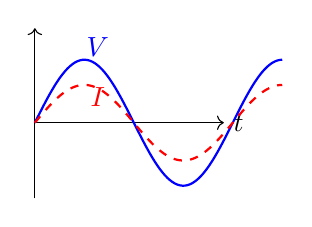
\begin{tikzpicture}[scale=0.8]
\draw[->] (0,-1.2) -- (0,1.5);
\draw[->] (0,0) -- (3,0) node[right] {$t$};
\draw[thick, blue] plot[domain=0:2.5*pi, samples=100] (\x/2, {sin(\x r)});
\draw[thick, red, dashed] plot[domain=0:2.5*pi, samples=100] (\x/2, {0.6*sin(\x r)});
\node[blue] at (1,1.2) {$V$};
\node[red] at (1,0.4) {$I$};
\end{tikzpicture}
\end{minipage}
\end{center}
\end{solutionbox}

\begin{mnemonicbox}
``Resistor Refuses Phase Shift''
\end{mnemonicbox}

%----------------------------------------
\section*{Question 5(b) [4 marks]}
\textbf{Define: Impedance, Phase angle, Power factor, Reactive power.}

\begin{solutionbox}
\begin{center}
\begin{tabular}{|l|p{6cm}|l|}
\hline
\textbf{Term} & \textbf{Definition} & \textbf{Formula} \\
\hline
Impedance & Total opposition to current flow ($Z$). & $Z = \sqrt{R^2 + X^2}$ \\
\hline
Phase Angle & Angle difference between $V$ and $I$. & $\phi = \tan^{-1}(X/R)$ \\
\hline
Power Factor & Cosine of phase angle causing active power. & $PF = \cos\phi = R/Z$ \\
\hline
Reactive Power & Power oscillating between source and load. & $Q = VI \sin\phi$ \\
\hline
\end{tabular}
\end{center}
\end{solutionbox}

\begin{mnemonicbox}
``Impedance Phase Power Quadrature''
\end{mnemonicbox}

%----------------------------------------
\section*{Question 5(c) [7 marks]}
\textbf{Enlist different protective device and explain construction and working of any one (MCB).}

\begin{solutionbox}
\textbf{Devices}: Fuse, MCB, MCCB, ELCB, Relay.

\textbf{MCB (Miniature Circuit Breaker):}
\begin{itemize}
\item \textbf{Construction}: Contacts, Arc chute, Bimetallic strip (Thermal), Magnetic coil (Magnetic).
\end{itemize}

\textbf{Working Principle:}
\begin{enumerate}
\item \textbf{Overload}: Bimetallic strip heats up and bends, unlatching the mechanism (Slow).
\item \textbf{Short Circuit}: High current in magnetic coil creates strong field, tripping instantly (Fast).
\end{enumerate}

\textbf{Block Diagram:}
\begin{center}
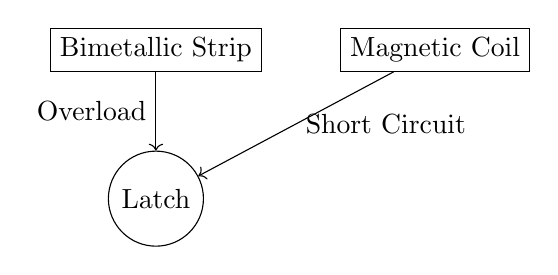
\begin{tikzpicture}
\node[draw, rectangle] (Strip) {Bimetallic Strip};
\node[draw, rectangle, right=of Strip] (Coil) {Magnetic Coil};
\node[draw, circle, below=of Strip] (Mech) {Latch};
\draw[->] (Strip) -- (Mech) node[midway, left] {Overload};
\draw[->] (Coil) -- (Mech) node[midway, right] {Short Circuit};
\end{tikzpicture}
\end{center}
\end{solutionbox}

\begin{mnemonicbox}
``MCB Magnetically Controls Both''
\end{mnemonicbox}

%----------------------------------------
\section*{Question 5(a OR) [3 marks]}
\textbf{Derive equation of AC current passing through pure inductor.}

\begin{solutionbox}
\textbf{Given}: $v = V_m \sin(\omega t)$, $v = L \frac{di}{dt}$

\textbf{Derivation}:
\[di = \frac{v}{L} dt = \frac{V_m}{L} \sin(\omega t) dt\]
\[i = \int \frac{V_m}{L} \sin(\omega t) dt = -\frac{V_m}{\omega L} \cos(\omega t)\]
\[i = \frac{V_m}{\omega L} \sin(\omega t - 90^\circ)\]

\textbf{Conclusion}: Current lags voltage by $90^\circ$. $X_L = \omega L$.
\end{solutionbox}

\begin{mnemonicbox}
``Inductor Impedes, Current Lags''
\end{mnemonicbox}

%----------------------------------------
\section*{Question 5(b OR) [4 marks]}
\textbf{Explain concept of power and power triangle in AC circuit.}

\begin{solutionbox}
\textbf{Power Types:}
\begin{itemize}
\item \textbf{Active ($P$)}: $VI \cos\phi$ (Watts) - Useful work.
\item \textbf{Reactive ($Q$)}: $VI \sin\phi$ (VAR) - Field maintenance.
\item \textbf{Apparent ($S$)}: $VI$ (VA) - Total rating.
\end{itemize}

\textbf{Power Triangle:}
\begin{center}
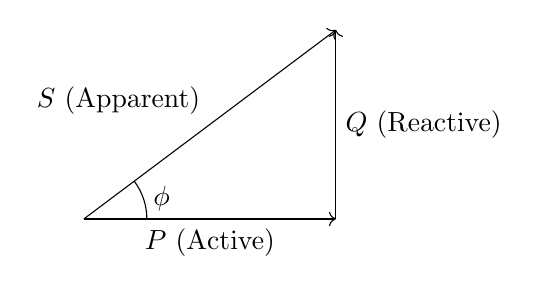
\begin{tikzpicture}[scale=0.8]
\draw[->] (0,0) -- (4,0) node[midway, below] {$P$ (Active)};
\draw[->] (4,0) -- (4,3) node[midway, right] {$Q$ (Reactive)};
\draw[->] (0,0) -- (4,3) node[midway, above left] {$S$ (Apparent)};
\draw (1,0) arc (0:36.8:1) node[midway, right] {$\phi$};
\end{tikzpicture}
\end{center}

$S^2 = P^2 + Q^2$. Power Factor $\cos\phi = P/S$.
\end{solutionbox}

\begin{mnemonicbox}
``Power Triangle: Please Qualify Students''
\end{mnemonicbox}

%----------------------------------------
\section*{Question 5(c OR) [7 marks]}
\textbf{Explain wiring of lamp control from one place and staircase type.}

\begin{solutionbox}
\textbf{1. One Place Control:}
Simple series circuit with Switch ($S$) and Lamp ($L$).
\\
\textbf{Diagram}: Live $\rightarrow$ Switch $\rightarrow$ Lamp $\rightarrow$ Neutral.

\textbf{2. Staircase Wiring (Two way control):}
Uses two SPDT (Single Pole Double Throw) switches.

\textbf{Diagram:}
\begin{center}
\begin{circuitikz}[scale=1.0]
\draw (0,0) node[left]{Live} to[short] (1,0); 
% Switch 1
\draw (1,0) -- (1.5, 0.5) node[above]{A1};
\draw (1,0) -- (1.5, -0.5) node[below]{B1};
% Switch 2
\draw (4.5,0) -- (4, 0.5) node[above]{A2};
\draw (4.5,0) -- (4, -0.5) node[below]{B2};
\draw (4.5,0) to[lamp] (6,0) node[right]{Neutral};
% Wires
\draw (1.5, 0.5) -- (4, 0.5);
\draw (1.5, -0.5) -- (4, -0.5);
\end{circuitikz}
\end{center}

\textbf{Working}: The lamp can be switched ON/OFF from either switch independent of the other's position.
\end{solutionbox}

\begin{mnemonicbox}
``Two-way Toggles, Two Places''
\end{mnemonicbox}

\end{document}
